\section{Basic Concepts}

\noindent
A {\color{blue}\it differential equation} is an equation that contains one or more
derivatives of an unknown function. The {\color{blue}\it order\/} of a
differential equation is the order of the highest
derivative that it contains. A differential equation is an
{\color{blue}\it ordinary differential equation\/} if it involves an unknown
function of only one variable, or a {\color{blue}\it partial differential
equation\/} if it involves partial derivatives of a function of more
than one variable. For now we'll consider only ordinary differential
equations, and we'll just call them {\color{blue}\it differential equations.\/}

Throughout this text, all variables and constants are real unless it's
stated otherwise. We'll usually use $x$ for the independent variable
unless the independent variable is time; then we'll use $t$.

The simplest differential equations are first order equations of the
form
$$
{dy\over dx}=f(x) \mbox{\quad or, equivalently, \quad}y'=f(x),
$$
where $f$  is a known function of $x$. We already know from calculus
how to find functions that satisfy this kind of equation. For example,
if
$$
y'=x^3,
$$
then
$$
y=\int x^3\, dx={x^4\over4}+c,
$$
 where $c$ is an arbitrary constant.  If $n>1$
we can find functions $y$ that satisfy
equations of the form
\begin{equation} \label{eq:1.2.1}
y^{(n)}=f(x)
\end{equation}
by repeated integration. Again, this is a calculus problem.

Except for illustrative purposes in this section, there's no need to
consider differential equations like \eqref{eq:1.2.1}. We'll
usually consider differential equations that can be written as
\begin{equation} \label{eq:1.2.2}
y^{(n)}=f(x,y,y', \dots,y^{(n-1)}),
\end{equation}
where at least one of the functions $y$, $y'$, \dots, $y^{(n-1)}$ actually
appears on the right. Here are some examples:
$$
\begin{array}{rcll}
\dst{dy\over dx}-x^2&=&0&\mbox{ (first order)},  \\[2\jot]
\dst{dy\over dx}+2xy^2&=&-2&\mbox{ (first order)},   \\[2\jot]
\dst{d^2y\over dx^2}+2\dst{dy\over dx}+y&=&2x&\mbox{ (second order)},
\\[2\jot]
xy'''+y^2&=&\sin x  &\mbox{ (third order)},
\\[2\jot] y^{(n)}+xy'+3y&=&x&\mbox{ ($n$-th order)}.
\end{array}
$$
Although none of these equations is  written as in
\eqref{eq:1.2.2}, all of them {\color{blue}\it can\/} be written in this form:
$$
\begin{array}{rcl}
y'&=&x^2,  \\
y'&=&-2-2xy^2,   \\
y''&=&2x-2y'-y,  \\
y'''&=&\dst{\sin x-y^2\over x},
\\[2\jot] y^{(n)}&=&x-xy'-3y.
\end{array}
$$

\boxit{Solutions of Differential Equations}

\noindent
A {\color{blue}\it solution\/} of a differential equation is a function that
satisfies the differential equation on some open interval;   thus, $y$
is a solution of \eqref{eq:1.2.2} if $y$ is $n$ times differentiable and
$$
y^{(n)}(x)=f(x,y(x),y'(x), \dots,y^{(n-1)}(x))
$$
for all $x$ in some open interval $(a,b)$. In this case, we also say
that $y$ {\color{blue}\it is a solution of \eqref{eq:1.2.2} on\/} $(a,b)$. Functions
that satisfy a differential equation at isolated points are not
interesting. For example, $y=x^2$ satisfies
$$
xy'+x^2=3x
$$
if and only if $x=0$ or $x=1$, but it's not a solution of this
differential equation because it does not satisfy the equation on an
open interval.

The graph of a solution of a differential equation is  a {\color{blue}\it
solution curve\/}. More generally, a curve $C$ is said to be an {\color{blue}\it
integral curve\/} of a differential equation if every function
$y=y(x)$ whose graph is a segment of $C$ is a solution of the
differential equation. Thus, any solution curve of a differential
equation is an integral curve, but an integral curve need not be a
solution curve.

\begin{example}
\label{example:1.2.1} \rm
If $a$ is any positive constant,  the circle
\begin{equation} \label{eq:1.2.3}
x^2+y^2=a^2
\end{equation}
is an integral curve of
\begin{equation} \label{eq:1.2.4}
y'=-{x\over y}.
\end{equation}
To see this, note that the only functions whose graphs are segments of
\eqref{eq:1.2.3} are
$$
y_1=\sqrt{a^2-x^2}\mbox{\quad and \quad} y_2=-\sqrt{a^2-x^2}.
$$
We leave it to you to verify that these functions both satisfy
\eqref{eq:1.2.4} on the open interval $(-a,a)$. However, \eqref{eq:1.2.3} is
not a solution
curve of \eqref{eq:1.2.4}, since it's not the graph of a function.
\end{example}

\begin{example}\label{example:1.2.2} \rm
Verify that
\begin{equation} \label{eq:1.2.5}
y={x^2\over3}+{1\over x}
\end{equation}
is a solution of
\begin{equation} \label{eq:1.2.6}
xy'+y=x^2
\end{equation}
 on $(0,\infty)$ and on $(-\infty,0)$.
\end{example}

\solution
Substituting \eqref{eq:1.2.5} and
$$
y'={2x\over3} - {1\over x^2}
$$
into \eqref{eq:1.2.6}  yields
$$
xy'(x)+y(x)=x \left({2x\over3} - {1\over x^2}\right)+
\left({x^2\over3}+{1\over x}\right)=x^2
$$
for all $x\ne0$. Therefore $y$ is a solution of \eqref{eq:1.2.6}
on $(-\infty,0)$ and $(0,\infty)$.
 However, $y$ isn't  a solution of the differential
equation on any open interval that contains $x=0$, since  $y$ is
not defined at  $x=0$.

Figure~\ref{figure:1.2.1} shows the graph
of \eqref{eq:1.2.5}. The
part
of the graph of \eqref{eq:1.2.5} on $(0,\infty)$ is a solution curve of
\eqref{eq:1.2.6}, as is the part of the graph on $(-\infty,0)$.

\begin{example}\label{example:1.2.3} \rm
 Show that if $c_1$ and $c_2$ are constants then
\begin{equation} \label{eq:1.2.7}
y=(c_1+c_2x)e^{-x}+2x-4
\end{equation}
 is a solution of
\begin{equation} \label{eq:1.2.8}
y''+2y'+y=2x
\end{equation}
 on $(-\infty,\infty)$.
\end{example}

\begin{figure}[thp]
  \centering
  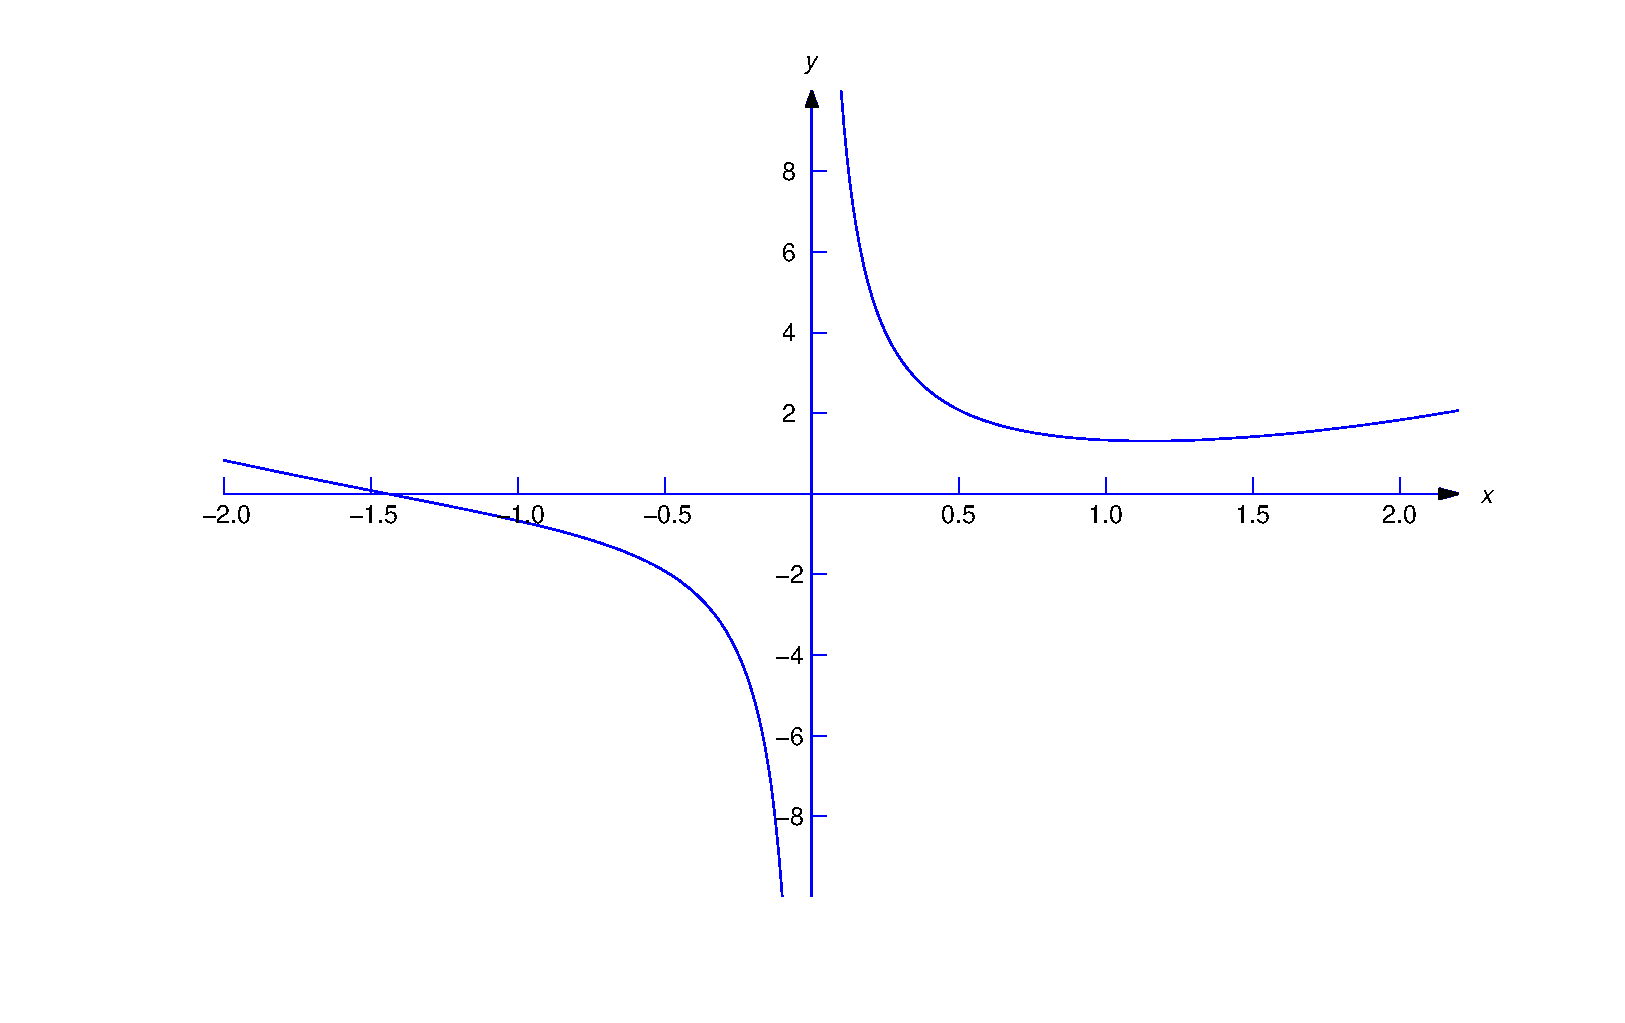
\includegraphics[bb=-78 148 689 643,width=5.67in,height=3.66in,keepaspectratio]{fig010201}
\color{blue}
  \caption{$y=\dst{\frac{x^{2}}{3}+\frac{1}{x}}$}
  \label{figure:1.2.1}
\end{figure}

\solution Differentiating \eqref{eq:1.2.7} twice yields
$$
y'=-(c_1+c_2x)e^{-x}+c_2e^{-x}+2
$$
 and
$$
y''=(c_1+c_2x)e^{-x}-2c_2e^{-x},
$$
so
\begin{eqnarray*}
y''+2y'+y&=&(c_1+c_2x)e^{-x}-2c_2e^{-x}\\
&&+2\left[-(c_1+c_2x)e^{-x}+c_2e^{-x}+2\right]\\
&&+(c_1+c_2x)e^{-x}+2x-4\\
&=&(1-2+1)(c_1+c_2x)e^{-x}+(-2+2)c_2e^{-x}\\ &&+4+2x-4=2x
\end{eqnarray*}
for all values of $x$.
Therefore $y$ is a solution of \eqref{eq:1.2.8} on $(-\infty,\infty)$.

\begin{example}\label{example:1.2.4} \rm
Find all solutions of
\begin{equation} \label{eq:1.2.9}
y^{(n)}=e^{2x}.
\end{equation}
\end{example}

\solution Integrating \eqref{eq:1.2.9} yields
$$
y^{(n-1)}={e^{2x}\over2}+k_1,
$$
 where $k_1$ is a constant. If $n\ge2$,
integrating again yields
$$
y^{(n-2)}={e^{2x}\over4}+k_1x+k_2.
$$
If $n\ge3$, repeatedly integrating yields
\begin{equation} \label{eq:1.2.10}
y={e^{2x}\over2^n}+k_1{x^{n-1}\over (n-1)!}+k_2{x^{n-2}\over
(n-2)!}+\cdots+k_n,
\end{equation}
 where $k_1$, $k_2$, \dots, $k_n$ are constants.
This shows that every solution of \eqref{eq:1.2.9} has the form
\eqref{eq:1.2.10}
for some choice of the constants $k_1$, $k_2$, \dots, $k_n$.
On the other hand, differentiating \eqref{eq:1.2.10}  $n$ times shows
that if
$k_1$, $k_2$, \dots, $k_n$ are arbitrary constants, then the function $y$
in
\eqref{eq:1.2.10} satisfies \eqref{eq:1.2.9}.

Since the constants $k_1$, $k_2$, \dots, $k_n$  in \eqref{eq:1.2.10}
are arbitrary, so are the constants
$${k_1\over (n-1)!},\, {k_2\over(n-2)!},\, \cdots, \, k_n.$$
 Therefore Example~\ref{example:1.2.4} actually shows that all
solutions of \eqref{eq:1.2.9}  can be written as
$$
y={e^{2x}\over2^n}+c_1+c_2x+\cdots+c_nx^{n-1},
$$
 where we  renamed the arbitrary constants in
\eqref{eq:1.2.10} to obtain a simpler formula. As a
general rule, arbitrary constants appearing in solutions  of differential
equations should be simplified if possible. You'll see examples
of this throughout the text.

\boxit{Initial Value Problems}

\noindent
In Example~\ref{example:1.2.4} we saw that the differential equation
$y^{(n)}=e^{2x}$ has an infinite family of solutions that depend upon
the $n$ arbitrary constants $c_1$, $c_2$, \dots, $c_n$. In the absence of
additional conditions, there's no reason to prefer one solution of a
differential equation over another. However, we'll often be
interested in finding a solution of a differential equation that
satisfies one or more specific conditions. The next example
illustrates this.

\begin{example}\label{example:1.2.5} \rm
 Find a solution of
$$
y'=x^3
$$
 such that $y(1)=2$.
\end{example}

\solution  At the beginning of this section we saw
that the  solutions of $y'=x^3$ are
$$
y={x^4\over4}+c.
$$
 To determine a value of $c$ such that $y(1)=2$,
we set $x=1$ and $y=2$ here to obtain
$$
2=y(1)={1\over4}+c,\mbox{\quad so \quad}c={7\over4}.
$$
 Therefore the required solution is
$$
y={x^4+7\over4}.
$$

Figure~\ref{figure:1.2.2} shows
the graph  of this solution.
Note that imposing the  condition $y(1)=2$ is equivalent to requiring
 the graph of $y$ to pass through the point $(1,2)$.

 We can rewrite the problem considered in Example~\ref{example:1.2.5}
more briefly as
$$
y'=x^3,\quad y(1)=2.
$$
 We call this an {\color{blue}\it initial value problem\/}.
The requirement $y(1)=2$ is an {\color{blue}\it initial condition}.
 Initial value problems can also be
posed for higher order differential equations.  For example,
\begin{equation} \label{eq:1.2.11}
y'' - 2y'+3y=e^x, \quad y(0)=1, \quad y'(0)=2
\end{equation}
is  an initial value problem for a second order differential
equation where $y$ and $y'$ are required to have specified values at
 $x=0$. In general, an initial value
problem for an $n$-th order differential equation requires $y$ and its
first $n-1$ derivatives to have specified values at some point $x_0$.
These requirements are the {\color{blue}\it initial conditions\/}.

\begin{figure}[H]
  \centering
  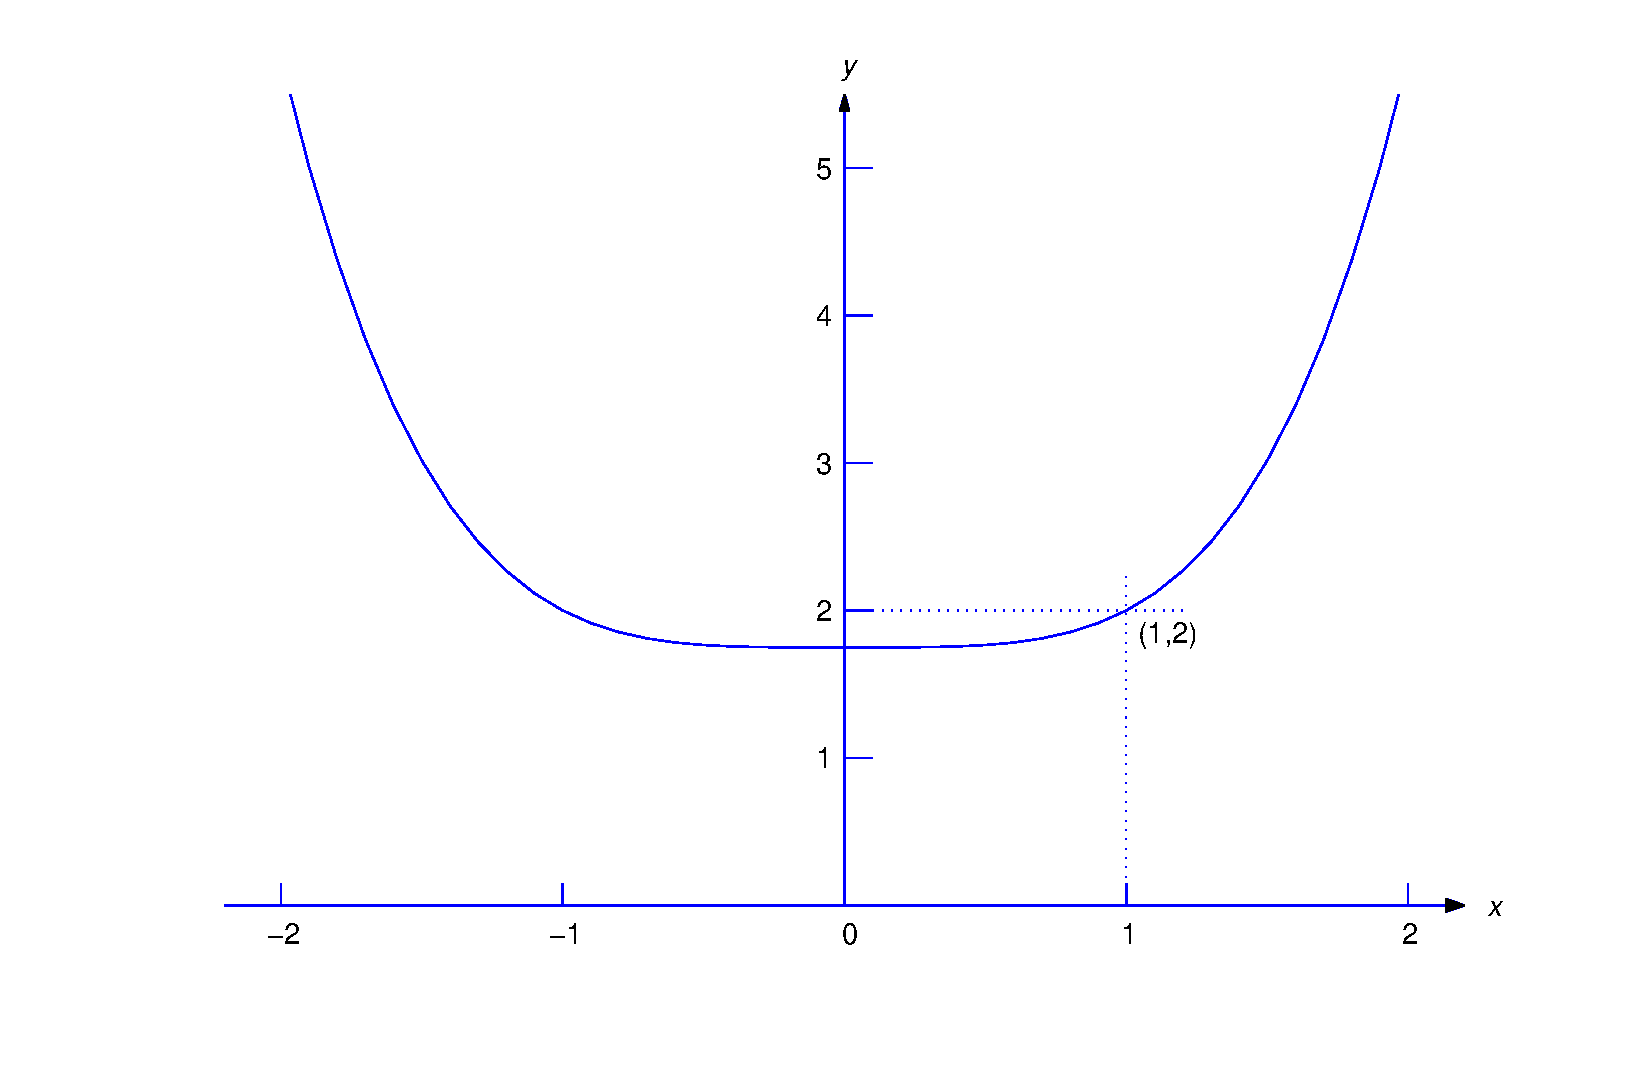
\includegraphics[bb=-78 148 689 643,width=5.67in,height=3.66in,keepaspectratio]{fig010202}
\color{blue}
  \caption{$y=\dst{\frac{x^{2}+7}{4}}$ }
  \label{figure:1.2.2}
\end{figure}

We'll denote an initial value problem for a differential equation by
writing the initial conditions after the equation, as in
\eqref{eq:1.2.11}. For example, we would write an initial value problem
for \eqref{eq:1.2.2} as
\begin{equation} \label{eq:1.2.12}
y^{(n)}=f(x,y,y', \dots,y^{(n-1)}),\, y(x_0)=k_0,\,
y'(x_0)=k_1,\, \dots,\, y^{(n-1)}=k_{n-1}.
\end{equation}
Consistent with our earlier definition of a solution of the
differential equation in \eqref{eq:1.2.12}, we say that $y$ is a solution
of the initial value problem \eqref{eq:1.2.12}  if $y$ is $n$ times
differentiable and
$$
y^{(n)}(x)=f(x,y(x),y'(x), \dots,y^{(n-1)}(x))
$$
for all $x$ in some open interval $(a,b)$  that contains $x_0$,
and  $y$ satisfies the initial conditions in \eqref{eq:1.2.12}. The
largest open interval that contains $x_0$ on which $y$ is defined and
satisfies the differential equation is  the {\color{blue}\it interval of
validity} of $y$.

\begin{example}\label{example:1.2.6} \rm
In Example~\ref{example:1.2.5} we saw that
\begin{equation} \label{eq:1.2.13}
y={x^4+7\over4}
\end{equation}
is a solution of the initial value problem
$$
y'=x^3,\quad y(1)=2.
$$
Since the function in \eqref{eq:1.2.13} is defined for all $x$, the
interval of validity of this solution is $(-\infty,\infty)$.
\end{example}

\begin{example}\label{example:1.2.7} \rm
In Example~\ref{example:1.2.2} we verified that
\begin{equation} \label{eq:1.2.14}
y={x^2\over3}+{1\over x}
\end{equation}
is a solution of
$$
xy'+y=x^2
$$
on $(0,\infty)$ and on $(-\infty,0)$. By evaluating \eqref{eq:1.2.14} at
$x=\pm1$, you can see that \eqref{eq:1.2.14} is a solution of the initial
value problems
\begin{equation} \label{eq:1.2.15}
xy'+y=x^2,\quad y(1)={4\over3}
\end{equation}
and
\begin{equation} \label{eq:1.2.16}
xy'+y=x^2,\quad y(-1)=-{2\over3}.
\end{equation}
The interval of validity of \eqref{eq:1.2.14} as a solution of
\eqref{eq:1.2.15} is $(0,\infty)$, since this is the largest interval
that contains $x_0=1$ on which \eqref{eq:1.2.14} is defined. Similarly, the
interval of validity of \eqref{eq:1.2.14} as a solution of \eqref{eq:1.2.16}
is $(-\infty,0)$, since this is the largest interval that contains
$x_0=-1$ on which \eqref{eq:1.2.14} is defined.
\end{example}

\boxit{Free Fall Under Constant Gravity}

\noindent
The term {\color{blue}\it initial value problem}  originated in problems
of motion where the independent variable is $t$
(representing elapsed time), and the initial conditions
are the position and velocity of an object at the initial
(starting) time of an experiment.

\begin{example}\label{example:1.2.8} \rm
An object falls under the influence of gravity near Earth's
surface, where it can be assumed that the magnitude of the
acceleration due to gravity is a constant $g$.
\begin{alist}
\item % (a)
 Construct a mathematical model for the motion of the object in the
form of an initial value problem for a second order differential
equation, assuming that the altitude and velocity of the object at
time $t=0$ are known. Assume that gravity is the only force acting on
the object.
\item % (b)
 Solve the initial value problem derived in \part{a} to obtain the
altitude as a function of time.
\end{alist}
\end{example}

\solutionpart{a} Let $y(t)$ be the altitude of the object at time $t$.
 Since the acceleration of the object has
constant magnitude $g$ and is in the downward (negative) direction,
$y$ satisfies the second order equation
$$
y''=-g,
$$
where the prime now indicates differentiation with respect to $t$.
If $y_0$ and $v_0$ denote the altitude and velocity when
$t=0$, then $y$ is a solution of the initial value problem
\begin{equation} \label{eq:1.2.17}
y''=-g,\quad  y(0)=y_0,\quad y'(0)=v_0.
\end{equation}

\solutionpart{b}
Integrating \eqref{eq:1.2.17} twice yields
\begin{eqnarray*}
y'&=&-gt+c_1, \\
y&=&-{gt^2\over2}+c_1t+c_2.
\end{eqnarray*}
Imposing the initial conditions $y(0)=y_0$ and $y'(0)=v_0$ in these
two equations shows that $c_1=v_0$ and $c_2=y_0$. Therefore the
solution of the initial value problem \eqref{eq:1.2.17} is
$$
y=- {gt^2\over2}+v_0t+y_0.
$$

\exercises
\begin{exerciselist}
\item\label{exer:1.2.1}
Find the order of the   equation.

\begin{tabular}[t]{@{}p{168pt}@{}p{168pt}}
{\bf (a)}\   $\dst{d^2y\over dx^2}+2
{dy\over dx}\   {d^3y\over dx^3}+x=0$
& {\bf (b)}\   $y''-3y'+2y=x^7$\\[9pt]
{\bf (c)}\   $y'-y^7=0$
& {\bf (d)}\   $y''y-(y')^2=2$
\end{tabular}

\item\label{exer:1.2.2}
Verify that the  function is a solution of the
differential equation on some interval, for any choice of
the arbitrary constants appearing in the function.

\begin{alist}
\item % (a)
 $y=ce^{2x};     \quad y'=2y$
\item % (b)
 $y=\dst{x^2\over3}
+{c\over x};   \quad xy'+y=x^2$

\item %(c)
$y=\dst{1\over2}+ce^{-x^2};    \quad y'+2xy=x$

\item %(d)
$y=(1+ce^{-x^2/2});   (1-ce^{-x^2/2})^{-1}   \quad
2y'+x(y^2-1)=0$

\item %(e)
$y=\dst{\tan\left( {x^3\over3}+c\right)};     \quad
y'=x^2(1+y^2)$

\item %(f)
$y=(c_1+c_2x)e^x+\sin x+x^2;    \quad
y''-2y'+y=-2 \cos x+x^2-4x+2$

\item %(g)
$y=c_1e^x+c_2x+\dst{2\over x};     \quad
(1-x)y''+xy'- y=4(1-x-x^2)x^{-3}$

\item %(h)
$y=x^{-1/2}(c_1\sin x+c_2 \cos x)+4x+8$;     \newline
$x^2y''+xy'+\dst{\left(x^2-{1\over4}\right)}y=4x^3+8x^2+3x-2$
\end{alist}

\item\label{exer:1.2.3}
Find all solutions of the  equation.

\begin{tabular}[t]{@{}p{168pt}@{}p{168pt}}
{\bf (a)}\quad  $y'=-x$
& {\bf (b)}\quad  $y'=-x \sin x$\\
{\bf (c)}\quad  $y'=x \ln x$
& {\bf (d)}\quad  $y''=x \cos x$\\
{\bf (e)}\quad  $y''=2xe^x$
& {\bf (f)}\quad  $y''=2x+\sin x+e^x$\\
{\bf (g)}\quad  $y'''=-\cos x$
& {\bf (h)}\quad  $y'''=-x^2+e^x$\\
{\bf (i)}\quad  $y'''=7e^{4x}$&
\end{tabular}

\item\label{exer:1.2.4}
Solve the  initial value problem.

\begin{alist}
\item % (a)
 $y'=-xe^x, \quad y(0)=1$
\item % (b)
 $\dst{y'=x \sin x^2, \quad y\left({\sqrt{\pi\over2}}\right)=1}$

\item %(c)
$y'=\tan x, \quad y(\pi/4)=3$

\item %(d)
$y''=x^4, \quad y(2)=-1, \quad y'(2)=-1$

\item %(e)
$y''=xe^{2x}, \quad y(0)=7, \quad y'(0)=1$

\item %(f)
$y''=- x \sin x, \quad y(0)=1, \quad y'(0)=-3$

\item %(g)
$y'''=x^2e^x, \quad y(0)=1, \quad y'(0)=-2, \quad
y''(0)=3$

\item %(h)
$y'''=2+\sin 2x, \quad y(0)=1, \quad y'(0)=-6, \quad
y''(0)=3$

\item %(i)
$y'''=2x+1, \quad y(2)=1, \quad
y'(2)=-4, \quad y''(2)=7$
\end{alist}

\item\label{exer:1.2.5}
Verify that the  function is a solution of
the initial value problem.

\begin{alist}
\item %(a)
$y=x\cos x;     \quad y'=\cos x-y\tan x, \quad
y(\pi/4)=\dst{\pi\over4\sqrt{2}}$

\item %(b)
$\dst{y={1+2\ln x\over x^2}+{1\over2};     \quad
y'={x^2-2x^2y+2\over x^3},   \quad y(1)={3\over2}}$

\item %(c)
$y=\dst{\tan\left({x^2\over2}\right)};
\quad y'=x(1+y^2),   \quad y(0)=0$

\item %(d)
$\dst{y={2\over x-2};     \quad y'={-y(y+1)\over x}}, \quad
y(1)=-2$
\end{alist}

\item\label{exer:1.2.6}
Verify that the  function is a solution of
the initial value problem.

\begin{alist}
\item %(a)
$y=x^2(1+\ln x);     \quad y''=\dst{3xy'-4y\over x^2}, \quad
y(e)=2e^2, \quad y'(e)=5e$

\item %(b)
$y=\dst{x^2\over3}+x-1;     \quad y''=\dst{x^2-xy'+y+1\over
x^2}, \quad y(1)=\dst{1\over3}, \quad y'(1)=\dst{5\over3}$

\item %(c)
$y=(1+x^2)^{-1/2};     \quad
y''=\dst{(x^2-1)y-x(x^2+1)y'\over (x^2+1)^2}, \quad y(0)=1$,

$y'(0)=0$

\item %(d)
$y=\dst{x^2\over 1-x};    \quad y''=\dst{2(x+y)(xy'-y)\over x^3},
\quad y(1/2)=1/2, \quad y'(1/2)=3$
\end{alist}

\item\label{exer:1.2.7}
Suppose an object is launched from a point 320 feet
above the earth with an initial velocity of 128 ft/sec
upward, and  the only force acting on it thereafter is
gravity. Take $g=32$ ft/sec$^2$.

\begin{alist}
\item %(a)
Find the highest altitude attained by the object.

\item %(b)
Determine how long it takes for the object to fall to the
ground.
\end{alist}

\item\label{exer:1.2.8}
\setcounter{equation}{0}
Let $a$ be a nonzero real number.
\begin{alist}
\item % (a)
Verify that if $c$ is an arbitrary constant then
$$
y=(x-c)^a
\eqno{\rm (A)}
$$
is a solution of
$$
y'=ay^{(a-1)/a}
\eqno{\rm (B)}
$$
on $(c,\infty)$.
\item % (b)
Suppose $a<0$ or $a>1$. Can you think of a solution of
(B) that isn't of the form (A)?
\end{alist}

\item\label{exer:1.2.9}
Verify that
$$
y=
\left\{ \begin{array}{cl}
e^x-1,& x \ge 0, \\[6pt]
1-e^{-x},& x < 0, \end{array}\right.
$$
is a solution of
$$
y'=|y|+1
$$
on $(-\infty,\infty)$. \hint{Use the definition of derivative
at $x=0$.}

\item\label{exer:1.2.10}
\begin{alist}
\item %(a)
Verify that if $c$ is any real number then
$$
y=c^2+cx+2c+1
\eqno{\rm (A)}
$$
satisfies
$$
 y'={-(x+2)+\sqrt{x^2+4x+4y}\over2}
\eqno{\rm (B)}
$$
on some open interval. Identify the open interval.

\item %(b)
Verify that
$$
y_1={-x(x+4)\over4}
$$
also satisfies  (B) on some open interval, and
identify the open interval. (Note that $y_1$ can't be obtained
by selecting a value of $c$ in (A).)
\end{alist}

\end{exerciselist}
